%-------------------------------------------------------------------------------
% 请勿删除本注释
% Free Response Question 2
%
% 指引:
% 如在小问之前有通用问题描述,请放置于此
%-------------------------------------------------------------------------------
\begin{figure}[H]
\centering
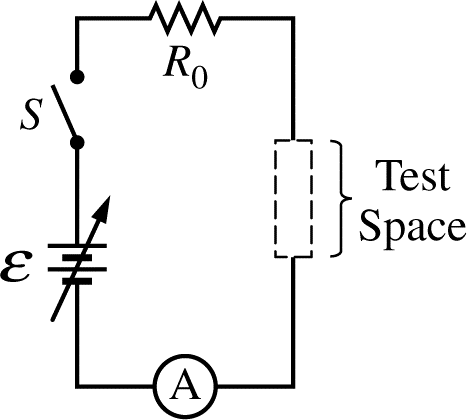
\includegraphics[scale=0.3]{images/img-020-046.png}
\end{figure}


\question
The circuit above consists of a variable DC power supply, an ammeter A, a switch $S$, and a resistor of unknown resistance $R_{0}$ connected in series with a test space into which different circuit elements can be placed. In order to determine $R_{0}$, a wire of negligible resistance is placed in the test space. The power supply is set at various potential differences, and the current in the circuit is measured. The data are shown below. % 请删除并替换本行,与上一行 \question 之间不要留空行


\begin{table}[H]
\centering
\begin{tabular}{|c|c|c|c|c|}
\hline$\varepsilon(\mathrm{V})$ & $2.00$ & $4.00$ & $6.00$ & $8.00$ \\
\hline Current $(\mathrm{mA})$ & $0.146$ & $0.310$ & $0.433$ & $0.577$ \\
\hline & & & & \\
\hline & & & & \\
\hline
\end{tabular}
\end{table}


\begin{parts}

%-------------------------------------------------------------------------------
% 请勿删除本注释
% Part (a)
%
% 指引:
% 如在小问之前有通用问题描述,请放置于此
%-------------------------------------------------------------------------------

\part
Indicate below which quantities should be graphed to yield a straight line that has a slope that could be used to calculate a numerical value for the resistance $R_{0}$. % 请删除并替换本行,与上一行 \part 之间不要留空行

Horizontal axis:\underline{\hspace{2cm}}

Vertical axis:\underline{\hspace{2cm}}

Use the remaining rows in the table above, as needed, to record any quantities that you indicated that are not given.

%-------------------------------------------------------------------------------
% 请勿删除本注释
% Part (b)
%
% 指引:
% 如在小问之前有通用问题描述,请放置于此
%-------------------------------------------------------------------------------

\part
Plot the straight line data points on the graph below. Clearly scale and label all axes, including units, if appropriate. Draw a straight line that best represents the data. % 请删除并替换本行,与上一行 \part 之间不要留空行

\begin{figure}[H]
\centering
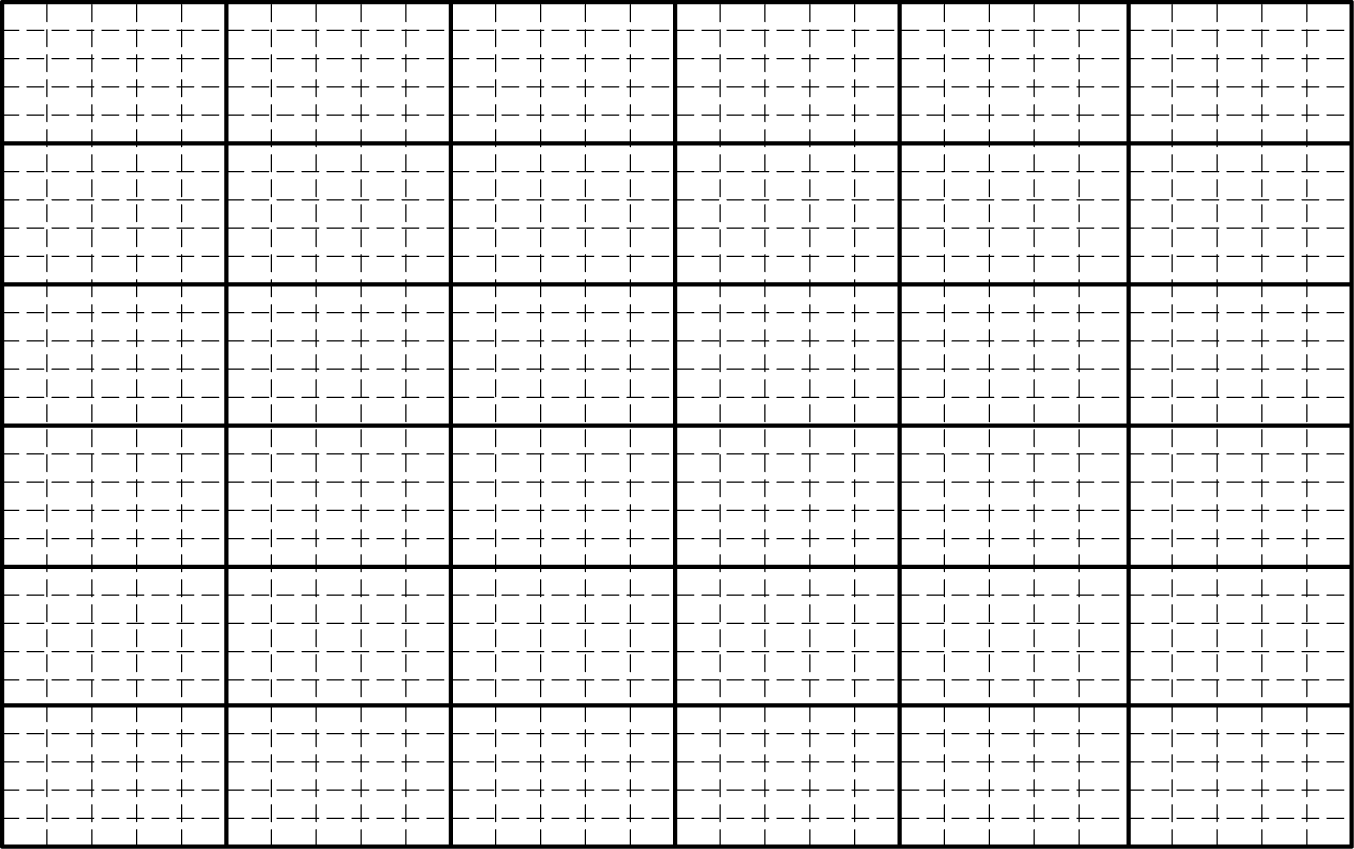
\includegraphics[scale=0.3]{images/img-021-047.png}
\end{figure}


%-------------------------------------------------------------------------------
% 请勿删除本注释
% Part (c)
%
% 指引:
% 如在小问之前有通用问题描述,请放置于此
%-------------------------------------------------------------------------------

\part
Using your straight line, calculate an experimental value for $R_{0}$. % 请删除并替换本行,与上一行 \part 之间不要留空行

%-------------------------------------------------------------------------------
% 请勿删除本注释
% Part (d)
%
% 指引:
% 如在小问之前有通用问题描述,请放置于此
%-------------------------------------------------------------------------------

\part
The power supply is set to $4.00 \mathrm{~V}$ and an uncharged, air-filled capacitor is placed in the test space. The switch is closed at time $t=0$, and the capacitor is allowed to fully charge. % 请删除并替换本行,与上一行 \part 之间不要留空行
\begin{subparts}
\subpart On the axes shown, sketch the current $I$ through the ammeter as a function of time $t$. Explicitly label any intercepts, asymptotes, maxima, or minima with numerical values or algebraic expressions, as appropriate.

\begin{figure}[H]
\centering
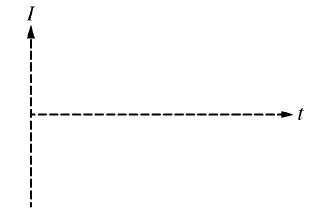
\includegraphics[scale=0.5]{images/2-d.png}
\end{figure}

\subpart It is determined that the time constant is $0.045 \mathrm{~s}$. The capacitor is charged to $4 \mathrm{~V}$. Calculate the energy stored in the capacitor.
\subpart The graph below shows the charge $Q$ on the capacitor as a function of time $t$. The capacitor is discharged, and a dielectric with dielectric constant $\kappa=2$ is inserted between the plates. The same charging procedure is repeated. On the graph below, sketch the curve showing the charge $Q$ on the dielectric-filled capacitor as a function of time $t$.

\begin{figure}[H]
\centering
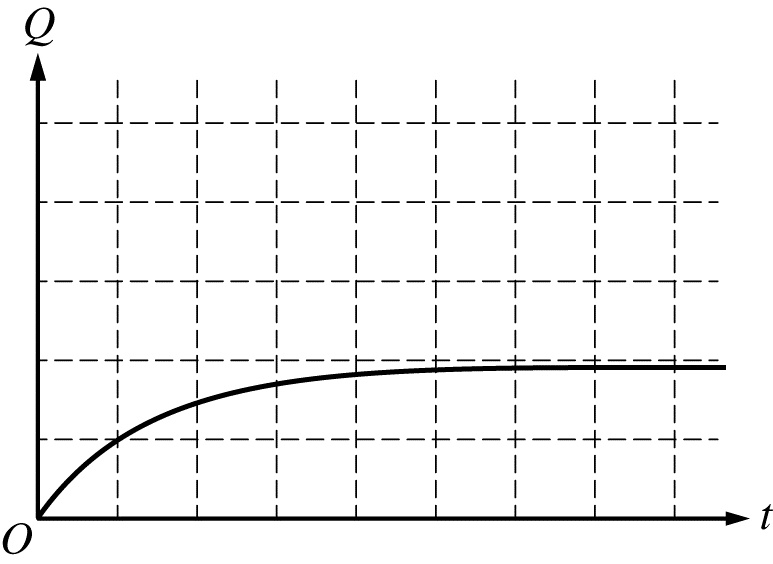
\includegraphics[scale=0.3]{images/img-022-049.png}
\end{figure}

\end{subparts}

\end{parts}
